\documentclass[fr]{../../../../../../eplexam}

\usepackage{../../../math-FSAB1103-exam}
\usepackage[SIunits]{../../../../../../eplunits}

\hypertitle{Math\'ematique}{3}{FSAB}{1103}{2017}{Août}
{Martin Braquet}
{Jean-François Remacle, Grégoire Winckelmans et Roland Keunings}

\section{}

On considère l'EDP suivante pour $u(x,t)$:
$$ 
\frac{\partial}{\partial x}(cu)+\frac{\partial u}{\partial t}=S
$$
où $$c=c(x)=\frac{c_0}{1+\frac{1}{2}\cos(2\pi\frac{x}{L})}$$ avec $c_0$ et $L$ constants.\\ 
Pour $s\geqslant0$, la condition initiale est $$u(s,0)=u_0\frac{s/L_0}{1+(s/L_0)^3}$$ avec $u_0$ et $L_0$ constants.\\
La condition limite est $u(0,\tau)=0$ pour $\tau\geqslant0$.

\begin{enumerate}
	
	\item Faites une esquisse (propre avec des axes chiffrés) de $c(x)/c_0$ en fonction de $x/L$. Avec uniquement cette information, faites alors une esquisse (propre avec des axes chiffrés) du réseau des caractéristiques dans le plan ($x/L,c_0t/L$) pour les régions A et B:
	\begin{itemize}
		\item Région A qui dépend de la condition initiale, dessiner les cas $s/L=0,1/4,1/2,3/4$.
		\item Région B qui dépend de la condition limite, dessiner les cas $c_0\tau/L=1/4$ et $1/2$..
	\end{itemize}
	
	\item Obtenir l'équation des caractéristiques dans la région A. Pour obtenir $s$ en fonction de $x$ et de $t$, i.e. $s=s(x,t)$, on doit résoudre numériquement une équation implicite, laquelle?
	
	\item On considère le cas particulier $S=cu/L$: obtenez la solution pour $u(x,t)$ dans la région A.
	
\end{enumerate}

\begin{solution}
	
\begin{enumerate}
	\item Par la règle de dérivation du produit, on écrit l'équation
	$$ 
	c(x)\frac{\partial u}{\partial x}+\frac{\partial u}{\partial t}=S-c'(x)u.
	$$ 
	
	On doit tracer la fonction 
	$$
		f(y)=\frac{1}{1+\frac{1}{2}\cos(2\pi y)},
	$$
	elle est périodique de période $T=1$ et vaut $2/3$ en $y=0$, $1$ en $y=1/4$, $2$ en $y=1/2$, $1$ en $y=3/4$. On peut ainsi obtenir le graphe ci-dessous.
	\begin{solfig}{c}{$c(x)/c_0$}
		\centering
		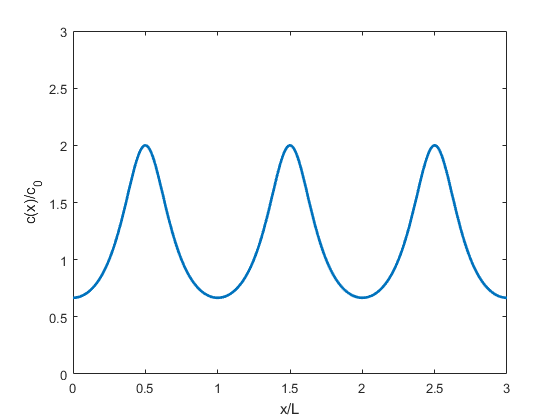
\includegraphics[scale = 0.6]{aout2017-1.png}
		%\caption{}
	\end{solfig}
	
	Pour obtenir le réseau de caractéristiques, on intègre la relation
	$Q \mbox{d} x= P \mbox{d} t$. La courbe $\Gamma$ est définie par morceaux et vaut l'union entre l'axe $t\geqslant0$ et l'axe $x\geqslant0$.
	
	Pour la région A, on intègre d'un point $(s,0)$ sur l'axe des $x$ positifs jusque $(x,t)$. On a donc
	$$ \int_s^x \mbox{d}\overline{x}=\int_0^t c(\overline{x}) \: \mbox{d}\overline{t}$$
	$$	\int_s^x \bigg(1+\frac{1}{2}\cos(2\pi \overline{x}/L )\bigg)\mbox{d}\overline{x}=c_0 t $$
	$$	\frac{x}{L}+\frac{1}{4\pi}\sin(2\pi x/L) -\frac{s}{L}-\frac{1}{4\pi}\sin(2\pi s/L) =\frac{c_0 t}{L} $$
	Cette égalité fournit le graphe de $\frac{c_0 t}{L}$ en fonction de $x/L$ pour la région A. Le graphe ci-dessous montre la fonction pour plusieurs valeurs de $s$.
	\begin{solfig}{c}{Esquisse des caractéristiques dans la région A}
		\centering
		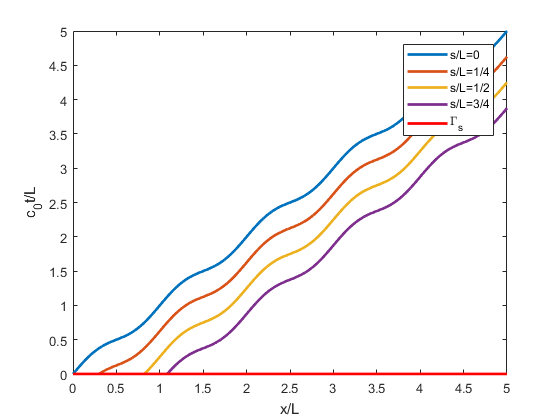
\includegraphics[scale = 0.6]{aout2017-2.png}
		%\caption{}
	\end{solfig}
	Pour tracer ce graphe, on remarque que l'on doit tracer la fonction
	$$ f(y)=y+\frac{1}{4\pi}\sin(2\pi y)+K$$
	avec $K$ une constante qui dépend de la valeur de $s$. C'est donc juste la somme de la fonction identité et d'un sinus de faible amplitude (oscillant entre $-1/(4\pi)$ et $1/(4\pi)$). Il faut ensuite trouver la valeur de $K$. Par exemple, pour $s/L=1/4$: $K=-\frac{s}{L}-\frac{1}{4\pi}\sin(2\pi s/L)=-1/4-\frac{1}{4\pi}$.\\
	
	Pour la région B, on intègre d'un point $(0,\tau)$ sur l'axe des $t$ positifs jusque $(x,t)$. On a donc
	$$ \int_0^x \mbox{d}\overline{x}=\int_\tau^t c(x) \:\mbox{d}\overline{t}$$
	$$		\frac{x}{L}+\frac{1}{4\pi}\sin(2\pi x/L)=\frac{c_0 t}{L}-\frac{c_0 \tau}{L} $$
	Cette égalité fournit le graphe de $\frac{c_0 t}{L}$ en fonction de $x/L$ pour la région B. Le graphe ci-dessous montre la fonction pour plusieurs valeurs de $\tau$.
	\begin{solfig}{c}{Esquisse des caractéristiques dans la région B}
		\centering
		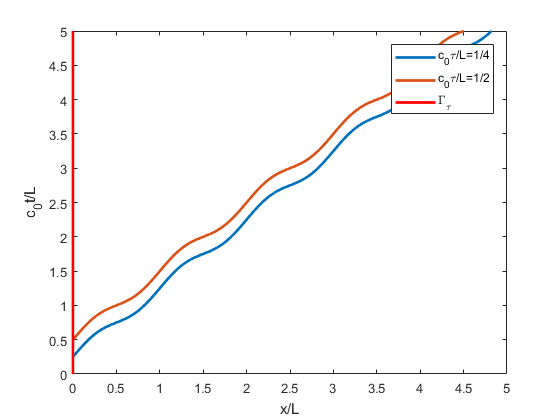
\includegraphics[scale = 0.6]{aout2017-3.png}
		%\caption{}
	\end{solfig}
	
	\item L'équation des caractéristiques établie avant est 
	$$\frac{x}{L}+\frac{1}{4\pi}\sin(2\pi x/L) -\frac{s}{L}-\frac{1}{4\pi}\sin(2\pi s/L) =\frac{c_0 t}{L} ,$$
	on ne peut pas isoler $s$ dans cette équation en $s$ et $\sin(s)$, c'est donc une équation implicite à résoudre numériquement.
	
	\item L'équation devient 
	$$ 
	c(x)\frac{\partial u}{\partial x}+\frac{\partial u}{\partial t}=\frac{cu}{L}-c'(x)u,
	$$ 
	on peut alors la résoudre en intégrant la relation $R \mbox{d} x= P \mbox{d} u$ le long des caractéristiques émanant de la courbe $\Gamma$ et situées dans la région A.
	$$
		\int_s^x (\frac{c(\overline{x})\overline{u}}{L}-c'(\overline{x})\overline{u}) \:\mbox{d} \overline{x}=\int_{u(s,0)}^{u(x,t)} c(\overline{x}) \: \mbox{d} \overline{u}
	$$
	$$
	\int_s^x (\frac{1}{L}-\frac{c'(\overline{x})}{c(\overline{x})}) \:\mbox{d} \overline{x}=\int_{u(s,0)}^{u(x,t)}  \frac{\mbox{d} \overline{u}}{\overline{u}}
	$$
	$$     \frac{x-s}{L}-\ln(\frac{c(x)}{c(s)})=\ln(\frac{u(x,t)}{u(s,0)})$$
	$$   \Rightarrow u(x,t)=u_0 e^\frac{x-s}{L} \frac{1+\frac{1}{2}\cos(2\pi x/L)}{1+\frac{1}{2}\cos(2\pi s/L)}\frac{s/L_0}{1+(s/L_0)^3}$$
	Cette solution contient encore la variable $s(x,t)$ qui doit être remplacée par la solution de l'équation implicite établie au point 2. 
	
\end{enumerate}	
	
\end{solution}


\section{}

On considère l'EDP suivante pour $u(x,t)$:
$$ 
\frac{\partial u}{\partial t}=\alpha \frac{\partial^2 u}{\partial x^2}+Q_0\cos(\frac{\pi}{2}\frac{x}{L})
$$
avec $\alpha>0$ et $Q_0$ constants.\\
Le domaine est borné: $0\leqslant x\leqslant L$.
La condition initiale est $$u(x,0)=u_0(2x/L-1)$$ avec $u_0>0$ constant.\\ Les conditions aux limites sont $\frac{\partial u}{\partial x}(0,t)=2u_0/L$ et $u(L,t)=u_0$.

\begin{enumerate}
	\item De quel type d'EDP s'agit-il, physiquement ET mathématiquement? Qu'est-ce qu'un temps \textit{court} pour une telle EDP : $0\leqslant t<<...$ ?
	\item La solution est de la forme $u(x,t) = R(x) + \Theta(x,t)$ avec $R$ la solution de régime et $\Theta$ la solution transitoire. 
	\begin{itemize}
		\item Obtenez d'abord $R$
		\item Obtenez ensuite $\Theta$ en utilisant la méthode de séparation des variables
	\end{itemize}
	
	\item On considère le cas particulier $$Q_0=(\pi/2)^2\frac{\alpha\: u_0}{L^2}.$$ Esquissez (proprement avec des axes chiffrés) le graphe attendu de $u/u_0$ en fonction de $x/L$ pour des temps différents: $t=0$ (CI), temps \textit{court}, temps \textit{moyen}, temps \textit{très long} (solution de régime).
\end{enumerate}


\begin{solution}
	
	\begin{enumerate}
		\item Il s'agit d'une équation parabolique (mathématiquement) et plus particulièrement de l'équation de diffusion (physiquement) avec un terme source, elle modélise par exemple un transfert de chaleur. Un temps court pour cette EDP, comme on le verra par la suite, est un temps pour lequel la solution n'a pas encore atteint sa valeur de régime, c'est-à-dire $t<L^2/\alpha$. En effet, $\alpha$ s'exprime en $m^2/s$, c'est donc la seule combinaison qui permet d'obtenir les mêmes unités que $t$. C'est peu probable qu'un facteur multiplicatif soit présent mais il est possible que $4L^2/(\pi^2\alpha)$ soit plus approprié en analysant la solution finale et le graphe de la solution.
		
		\item On remplace $u$ par $R(x)$ dans l'équation
		$$\alpha R''(x)+Q_0\cos\Big(\frac{\pi}{2}\frac{x}{L}\Big)=0 \Longrightarrow R(x)=Ax+B+\frac{Q_0}{\alpha}\Big(\frac{2L}{\pi}\Big)^2\cos\Big(\frac{\pi}{2}\frac{x}{L}\Big)\qquad A,B\in \Re$$
		On détermine A et B par les conditions limites:
		$$R'(0)=\frac{2u_0}{L}\Longrightarrow A=\frac{2u_0}{L}$$
		$$R(L)=AL+B=u_0\Longrightarrow B=-u_0$$
		$$\Longrightarrow R(x)=u_0(2x/L-1)+\frac{Q_0}{\alpha}\Big(\frac{2L}{\pi}\Big)^2\cos\Big(\frac{\pi}{2}\frac{x}{L}\Big)$$
		On calcule ensuite $\Theta(x,t)=X(x)T(t)$ en remplaçant $u$ par $\Theta$:
		$$\frac{T'}{T}=\frac{\alpha X''}{X}$$
		Puisque la partie gauche ne dépend que de $t$ et celle de droite ne dépend que de $x$, elle sont constantes et valent $0,k^2$ ou $-k^2$. Seul le cas $+k^2$ conduit à une solution non nulle:
		$$\frac{T'(t)}{T(t)}=k^2\Longrightarrow T(t)=Ce^-k^2 t \qquad C\in \Re$$
		$$\frac{\alpha X''(x)}{X(x)}=k^2 \Longrightarrow X(x)=D\cos\Big(\frac{k}{\sqrt{\alpha}}x\Big) +E\sin\Big(\frac{k}{\sqrt{\alpha}}x\Big) \qquad D,E\in \Re$$
		Puisque les conditions limites sont respectées par la solution de régime, ces conditions doivent être nulles pour la solution transitoire (sinon, les conditions aux frontières pour $u$ vaudraient 2 fois celles imposées par le problème). On résoud donc les conditions homogènes pour trouver C,D et E.
		$$  \frac{\partial \Theta}{\partial x}(0,t)=X'(0)T(t)=0\Longrightarrow E=0 $$
		$$\Theta(L,t)=X(L)T(t)=0\Longrightarrow CD\cos\Big(\frac{k}{\sqrt{\alpha}}L\Big)=0\Longrightarrow \frac{kL}{\sqrt{\alpha}}=\Big(n+\frac{1}{2}\Big)\pi$$
		$$k_n=\Big(n+\frac{1}{2}\Big)\frac{\sqrt{\alpha}\pi}{L}\qquad n=0,1,2,...$$
		On a donc comme solution transitoire
		$$\Theta(x,t)=\sum_{n=0}^{\infty} F_n e^{-k_n^2 t}\cos\Big(\Big(n+\frac{1}{2}\Big)\frac{\pi x}{L}\Big)$$
		avec $F_n=(CD)_n$.
		Il reste à trouver les constantes $F_n$ grâce à la condition initiale.
		$$\Theta(x,t=0)=u(x,0)-R(x)$$
		$$ \sum_{n=0}^{\infty} F_n \cos\Big(\Big(n+\frac{1}{2}\Big)\frac{\pi x}{L}\Big)=-\frac{Q_0}{\alpha}\Big(\frac{2L}{\pi}\Big)^2\cos\Big(\frac{\pi}{2}\frac{x}{L}\Big)  $$
		Par chance, la condition initiale est une fonction cosinus, les termes $F_n$ de la série de Fourier ne forment pas une suite infinie. Il suffit de prendre $$F_0=-\frac{Q_0}{\alpha}\Big(\frac{2L}{\pi}\Big)^2$$
		pour $n=0$ et $F_n=0$ pour $n>0$. Il n'est donc pas nécessaire d'utiliser la propriété d'orthogonalité des cosinus. Si vous avez quand même essayé d'intégrer en multipliant par le cosinus, vous auriez obtenu une somme de $\frac{1}{n}\sin(...x)$ et $\frac{1}{n+1}\sin(...x)$. Cette somme s'annule toujours sauf quand le dénominateur est nul ($n=0$) et on retombe sur le bon résultat.\\
		Finalement,
		$$ \Theta(x,t)= -\frac{Q_0}{\alpha}\Big(\frac{2L}{\pi}\Big)^2e^{-\frac{\pi^2\alpha}{4L^2} t}\cos\Big(\frac{\pi x}{2L}\Big)$$
		
		\item Avec le cas particulier, la solution finale vaut 
		$$\frac{u(x,t)}{u_0}=\frac{2x}{L}-1+\cos\Big(\frac{\pi x}{2L}\Big)\Big( 1-e^{-\frac{\pi^2\alpha}{4L^2} t} \Big)$$
		Les 2 graphes suivants présentent la solution.
		
		\begin{solfig}{c}{Solution $u/u_0$}
			\centering
			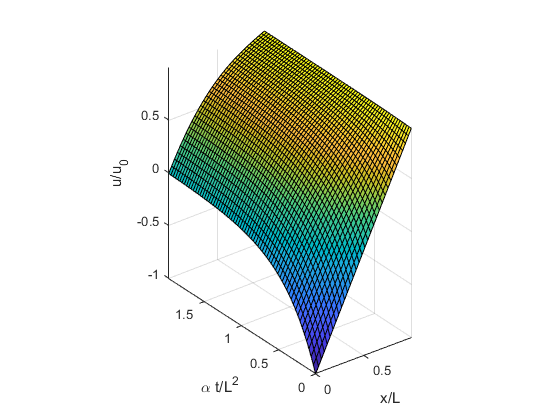
\includegraphics[scale = 0.6]{aout2017-4.png}
			%\caption{}
		\end{solfig}
		
		\begin{solfig}{c}{Solution $u/u_0$ pour des temps différents}
			\centering
			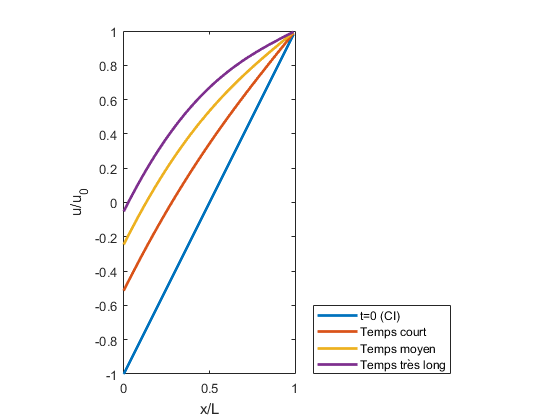
\includegraphics[scale = 0.8]{aout2017-5.png}
			%\caption{}
		\end{solfig}
	\end{enumerate}
	
	
	
\end{solution}


\section{}

On considère la fonction
$$f(z)=\frac{e^{-i/z}}{z}$$
\begin{enumerate}
	\item Calculez le résidu de $f(z)$ en $z=0$.
	\item Donnez les points singuliers de $f(z)$ et précisez leur type.
\end{enumerate}

\begin{solution}
	
	\begin{enumerate}
		\item On calcule le développement en série de Laurent de $f(z)$:
		$$ e^y=1+y+\frac{y^2}{2}+\frac{y^3}{6}+... $$
		$$ e^{-i/z}=1-\frac{i}{z}-\frac{1}{2z^2}+\frac{i}{6z^3}+... $$
		$$ \frac{e^{-i/z}}{z}=\frac{1}{z}-\frac{i}{z^2}-\frac{1}{2z^3}+\frac{i}{6z^4}+... $$
		Le résidu en $z=0$ est le coefficient du terme en $1/z$ de la série de Laurent et vaut donc 1. 
		\item $z=0$ est le seul point où $f(z)$ n'est pas dérivable. Puisqu'on peut trouver un voisinage dans lequel le point $z=0$ est le seul point singulier, ce point est un point singulier isolé. De plus, c'est un point singulier essentiel car $1/f(z)$ n'est pas bornée au voisinage de ce point:\\
		\begin{itemize}
			\item $f(z)$ n'est pas dérivable en 0 car elle n'est pas continue en ce point. Elle n'est pas bornée (et donc pas continue) en arrivant par le chemin $\Re(z)=0$ et $\Im (z)<0$: $$\lim_{y\rightarrow 0^-,x=0} f(z)=\lim_{y\rightarrow 0^-,x=0} \frac{e^{-i/(x+iy)}}{x+iy}=\lim_{y\rightarrow 0^-,x=0} \frac{e^{-1/y}}{iy}=\frac{e^{-1/0^-}}{i0^-}=-i\frac{\infty}{0^-}=+\infty\:i.$$
			\item $1/f(z)$ n'est pas bornée autour de 0 suivant le chemin $\Re(z)=0$ et $\Im (z)>0$: $$\lim_{y\rightarrow 0^+,x=0} 1/f(z)=\lim_{y\rightarrow 0^+,x=0} (x+iy)e^{i/(x+iy)}=\lim_{y\rightarrow 0^+,x=0}iye^{1/y}$$ $$=\lim_{y\rightarrow 0^+,x=0}\frac{ie^{1/y}}{1/y}\overset{\infty/\infty}{=}\lim_{y\rightarrow 0^+,x=0}\frac{-ie^{1/y}/y^2}{-1/y^2}=\lim_{y\rightarrow 0^+,x=0}ie^{1/0^+}=+\infty\:i.$$
			Il faut faire attention à vérifier la valeur de la fonction pour tout chemin passant par l'origine. En effet, la fonction tend vers 0 pour les 3 autres chemins principaux: venant de l'axe réel négatif, venant de l'axe réel positif et venant de l'axe imaginaire négatif.
		\end{itemize}
		
		Le fait que la série de Laurent ne soit pas limitée du côté des puissances négatives confirme qu'il ne s'agit pas d'un pôle.
		
		\begin{solfig}{c}{Graphe de $1/f(z)$ aux environs de $z=0$}
			\centering
			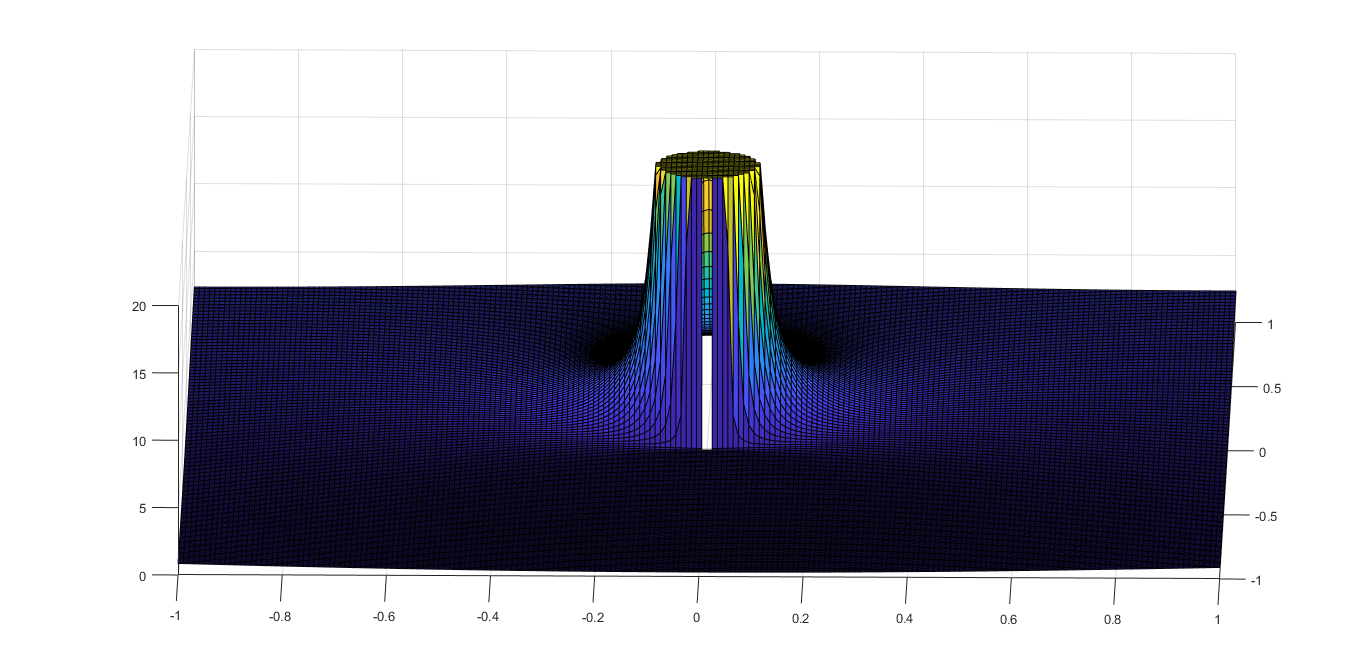
\includegraphics[scale = 0.3]{aout2017-7.png}
		\end{solfig}
		
		
		
	\end{enumerate}
	
\end{solution}


\section{}

Pour $m>0$, calculez l'intégrale suivante en utilisant le théorème des résidus:
$$\int_{0}^{\infty}{\frac{\cos(mx)}{1+x^2}dx}$$
Veillez à bien justifier toutes les étapes de calcul.\\
Note: les 5 lemmes de Jordan sont donnés.

\begin{solution}
	
	L'exercice est quasi identique à l'exercice 60 du syllabus écrit par Keunings. \\
	Calculons l'intégrale 
	$$\int_{C}{\frac{e^{imz}}{1+z^2}dz}$$
	avec $C$, le contour fermé en forme de demi-cercle illustré sur la figure ci-dessous.
	\begin{solfig}{c}{Contour d'intégration}
		\centering
		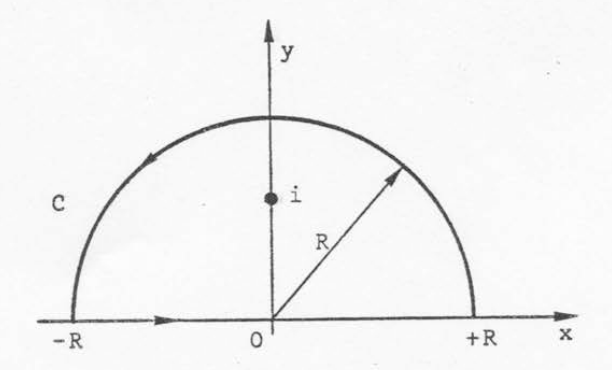
\includegraphics[scale = 0.4]{aout2017-6.png}
	\end{solfig}

	Ce contour entoure uniquement le pôle $z=i$. Le théorème des résidus s'énonce:\\
	Soit $f(z)$, une fonction holomorphe dans un domaine simplement connexe D sauf en un nombre fini de points $a_p$ qui sont des pôles ou des points singuliers essentiels de $f(z)$. Soit C une courbe fermée contenue dans D à l'intérieur de laquelle sont contenus tous les $a_p$. On a alors 
	$$\int_{C}f(z)dz=2\pi i \sum_{p=1}^{N}Res(a_p)$$
	où $Res(a_p)$ est le résidu de $f(z)$ relatif au point $a_p$.\\

	Ainsi, par ce théorème on a
	$$\int_{C}{\frac{e^{imz}}{1+x^2}dz}=2\pi i Res(i) $$
	$$\int_{-R}^R\frac{\cos(mx)}{1+z^2}dx+i\int_{-R}^R{\frac{\sin(mx)}{1+x^2}dx}+\int_{\Gamma}{\frac{e^{imz}}{1+z^2}dz}=2\pi i Res(i) $$
	avec $\Gamma$, la courbe $C$ dont on a enlevé le segment $[-R,R]$ sur l'axe réel. \\
	Le terme en sinus est nul car l'intégrant est impair et le domaine d'intégration est symétrique autour de l'origine.\\
	En faisant tendre $R$ à l'infini, le troisième terme est nul aussi par un des lemmes de Jordan:
	$$\lim_{R\rightarrow \infty}\int_{\Gamma}{\frac{e^{imz}}{1+x^2}dz}=\lim_{R\rightarrow \infty}\int_{\Gamma}{e^{imz}F(z)dz}$$
	avec $F(z)=1/(1+z^2)$. Le lemme de Jordan approprié précise que si $|F(z)|\leqslant M/R^k$ pour $z=Re^{i\theta}$, $M$ constante, $k>0$, alors 
	$$ \lim_{R\rightarrow \infty}\int_{\Gamma}{e^{imz}F(z)dz}=0 .$$
	On peut bien utiliser ce résultat car
	$$|F(z)|=\frac{1}{|1+R^2e^{2i\theta}|}<\frac{1}{|R^2||e^{2i\theta}|}=\frac{1}{R^2}=\frac{M}{R^k}$$
	avec $M=1$ et $k=2$.\\
	Finalement, 
	$$ \int_{-\infty}^\infty\frac{\cos(mx)}{1+x^2}dx=2\int_{0}^\infty\frac{\cos(mx)}{1+x^2}dx $$
	car l'intégrant est pair et le domaine d'intégration est symétrique autour de l'origine.\\
	On calcule ensuite le résidu:
	$$Res(i)= \lim_{z\rightarrow i}  \frac{e^{imz}}{i+z}=\frac{e^{-m}}{2i}$$
	 On obtient donc
	$$ 2\int_{0}^\infty\frac{\cos(mx)}{1+x^2}dx = 2\pi i \frac{e^{-m}}{2i}=\pi e^{-m} $$
	$$ \int_{0}^\infty\frac{\cos(mx)}{1+x^2}dx = \frac{\pi e^{-m}}{2}  $$
	
	
	
\end{solution}


\end{document}